\documentclass[main.tex]{subfiles} 

\begin{document}
\section*{Analyse}
\label{sec:2}

Hvordan ble undervisningen lagt opp for å skape god begrepsforståelse i naturfagstimene?
For å svare på dette, la oss se nærmere på hele undervisningssekvensen.
\newline
\newline
\subsection*{Aktivisering av forkunnskaper}
Både til den første og andre timen ble dialog initiert av læreren. Helklassesamtalene hadde preg av
IRE/F metoden, m.a.o lærer tar initiativ(I), elev responderer(R) og responsen blir evaluert(E) 
og/eller kommentert(F - feedback). Til den første timen rekker elevene opp hånda for å 
respondere. Det viser seg at det er noen få elever som er villig til å svare. 
\newline
\newline
\citeA[s. 176]{klet13} referer til et studie når hun viser til viktigheten av at lærerne 
legger til rette for \emph{systematisk trening, øvelse og bruk av naturfaglige begreper for å utvikle 
elevenes naturfaglige forståelse, inkludert repitisjon av sentrale begreper.}
\newline
\newline
Ved å være bevisst på at alle elevene skal ha kjennskap til 
begrepene som blir tatt opp og repetert, er det da nødvendig å få bekreftet at elevene innehar en 
overordnet forståelse. Det kan derfor være nødvendig å utpeke noen elever som ikke viser aktiv 
deltagelse i timen og frembringe deres respons. Hvis elevene ikke klarer å respondere på lærer 
initiativ, kan utspørringen av elevene vise hull i deres kunnskap. Ved å forutse elevsvar før elever 
i klassen blir initiert, kan misforståelser som ofte oppstår bli redegjortav læreren, og respons som 
ofte opptrer kan tas stilling til. Dette krever derimot en god del erfaring fra læreren sin side. I 
\citeA[s. ~401]{batp08} klassifiseres dette som \emph{knowledge of content and students, (KCS)}.
Over tid vil en lærer danne omfattende KCS og dette kan dermed bidra til å øke kvaliteten på
helklassesamtalene.
\newline
\newline
\citeA[s. ~136]{klet13} beskriver en god undervisningsseksens der lærere klarer å balansere mellom 
tilegnelses-, utprøvings-, og konsolideringssituasjoner. Ifølge Klette har norske klasserom ensidige 
tendenser i bruken av variert arbeidsmåter. Slik det kan ses fra figur \ref{fig:odeg10}, er det for 
eksempel lite konsolideringssituasjoner. Lærernes metalæringsaktiviteter regnes som særlig avgjørende 
for å sikre elevenes læring (\citeNP[s. 186]{klet13}). Derimot å bruke dette som et fast
organiserende prinsipp, blir sjelden gjennomført (\citeNP[s. 26]{odeg10}). Gjennom timen har 
aktivering av forkunnskaper, gjennom repitisjon og gjenbruk av begreper og gjennomgang av 
lekser, bæret preg av bevisst fokus på bruk av konsolideringssituasjoner/metalæringsaktiviteter.
Det var ingen appetittvekkere, og dette er noe som burde ha blitt inkludert 

\subsection*{Innføring av nytt tema}
Fra figuren \ref{fig:odeg10} kan vi også se at i en vanlig naturfagstime brukes mye tid på å utvikle 
nytt fagstoff.Det kan nok påstås at undervisningsopplegget hadde et preg av mange fagtermer, men 
fokuset i undervisningen var ikke på å innføre fagtermene, men isteden var fokuset å danne forståelse 
om begrepene og deres sammenhenger. 

\begin{figure}[h!]
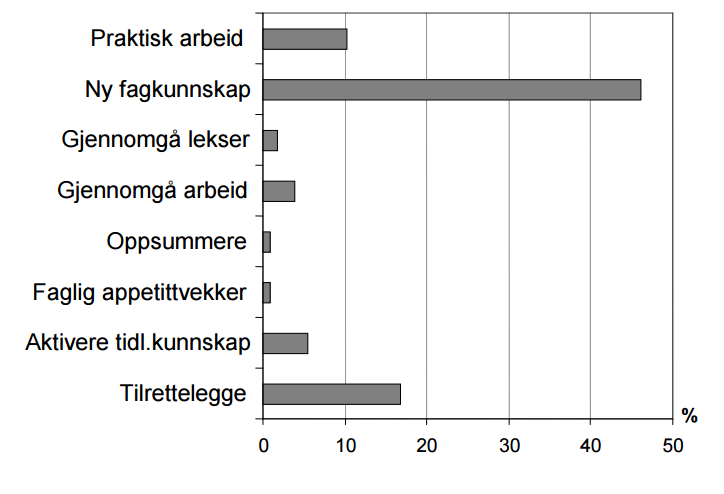
\includegraphics[scale = 0.6]{../figures/undervisnings_aktivitet.png}
\caption{Oversikt over naturfaglærernes undervisningstilbud til elevene fra PISA+ studie. Kilde: \protect\citeA{odeg10}.}
\label{fig:odeg10}
\end{figure}

%gode fagsentrerte samtaler mellom elever hvor elever brukte egne erfaringer
%og språket for å oppnå faglig forståelse, eller faglige samtaler med lærer som hjelper til å skape
%bro mellom praksis og teori 
%\citeA{odeg10}


%  ”inquiry-based science teaching” 
%\citeA{knai11}

\subsection*{Gruppe samtaler}
Siden resterende del av timen skal brukes til repetisjon, er det ikke nødvendig å 
prøve å finne svakheter i elevenes respons gjennom helklassesamtalen. For å finne slike svakheter 
ble gruppesamtalene en bedre plattform. I den forbindelse ble tokolonnenotatet tatt i bruk (se 
vedlegg : \ref{sec:tokolonnenotat}).

Evnen til abstrahering henger ifølge Vygotsky (\citeNP[s. 127]{bta98}) med begrepsundervisning, som en
form for vitenskapeliggjøring av hverdagsbegreper. Hvis elever ikke har god begrepsforståelse
kan de ende opp med å bruke naturvitenskapelige begreper i feil kontekst og danne feil 
forbindelser med begrepene. Dette avhenger av deres forkunnskaper. Ausubels kognitive bruer 
(\citeNP[s. 71]{math15}), hans teori om begrepslæring på høyere nivå og hvordan læreren best kan 
legge til rette for slik læring og bruk av begrepene,  handler om å danne forbindelser mellom 
undervisningsmateriell og relevante ideer i elevenes kognitive struktur.

\end{document}
